\documentclass{article}

\usepackage[T1]{fontenc}
\usepackage{polski}
\usepackage[utf8]{inputenc}

\usepackage{hyperref}
\usepackage[legalpaper, margin=1.2in]{geometry}

\usepackage{listings}
\usepackage[]{algorithm2e}

\title{AEM - Zadanie nr 1}
\author{Bartosz Sobkowiak 125342 Joanna Świda 138675}
\date{22.03.2020}

\usepackage{natbib}
\usepackage{graphicx}

\begin{document}

\maketitle
\section{Opis zadania}

    Rozważany problem to zmodyfikowana wersja problemu komiwojażera. Dany jest zbiór wierzchoł-
    ków i macierz symetrycznych odległości między nimi. Celem jest znalezienie najkrótszej ścieżki zamkniętej przechodzącej przez dokładnie 50\% wszystkich wierzchołków (w przypadku nieparzystej liczby wierzchołków zaokrąglamy w górę). Wybór wierzchołków do ścieżki jest elementem rozwiązania. Minimalizowane kryterium to długość zamkniętej ścieżki.
    


\section{Pseudokod}

\begin{algorithm}[H]
     \KwData{zbiór wierchołków, macierz odległości pomiędzy wierzchołkami}
     \KwResult{najrótsza ścieżka łącząca X\% wierzchołków}
     
    wybierz i dodaj punkt pierwszy\\
    znajdź punkt leżący najbliżej pierwszego i dodaj go jako punkt drugi\\
    \While{cykl zawiera mniej niż X\% wszystkich punktów}{
        \For{każdy pozostały punkt p} {
            oblicz długość cyklu cLen jeśli punkt p zostałby dodany do cyklu\\
        }\EndFor
        dodaj do cyklu punkt o najmniejszej wartośc cLen\\
        usuń ten punkt z listy pozostałych punktów\\
            }
\caption{Greedy Cycle}
\end{algorithm}

\vspace{10mm}

\begin{algorithm}[H]
     \KwData{zbiór wierchołków, macierz odległości pomiędzy wierzchołkami}
     \KwResult{najrótsza ścieżka łącząca X\% wierzchołków}
     
    wybierz i dodaj punkt pierwszy\\
    znajdź punkt leżący najbliżej pierwszego i dodaj go jako punkt drugi\\
    \While{cykl zawiera mniej niż X\% wszystkich punktów}{
        \For{każdy pozostały punkt p} {
            oblicz długość cyklu cLen jeśli punkt p zostałby dodany do cyklu\\
            oblicz żal dla danego punktu\\
        }\EndFor
        dodaj do cyklu rozwiązanie z największym żalem\\
        usuń punkt z listy pozostałych punktów\\
            }
\caption{Greedy Cycle with K-regret}
\end{algorithm}



\section{Wyniki obliczeń i wizualizacje}

\begin{table}[h!]
\centering
\begin{tabular}{ |c|c|c|c| } 
 \hline
 Zbiór & Min & Max & Avg \\ 
  \hline
 kroA$_{100}$ & 11284 & 16157 & 14313 \\ 
  \hline
 kroB$_{100}$ & 10417 & 20202 & 14169 \\ 
 \hline
\end{tabular}
\caption{Algorytm zachłanny - Greedy Cycle}
\end{table}

\begin{table}[h!]
\centering
\begin{tabular}{ |c|c|c|c| } 
 \hline
 Zbiór & Min & Max & Avg \\ 
  \hline
 kroA$_{100}$ & 18679 & 24313 & 21710 \\ 
  \hline
 kroB$_{100}$ & 19830 & 23675 & 21118 \\ 
 \hline
\end{tabular}
\caption{Algorytm z żalem - Greedy Cycle with K-regret}
\end{table}

\begin{figure}[h!]
  \centering
  \begin{minipage}[b]{0.8\textwidth}
    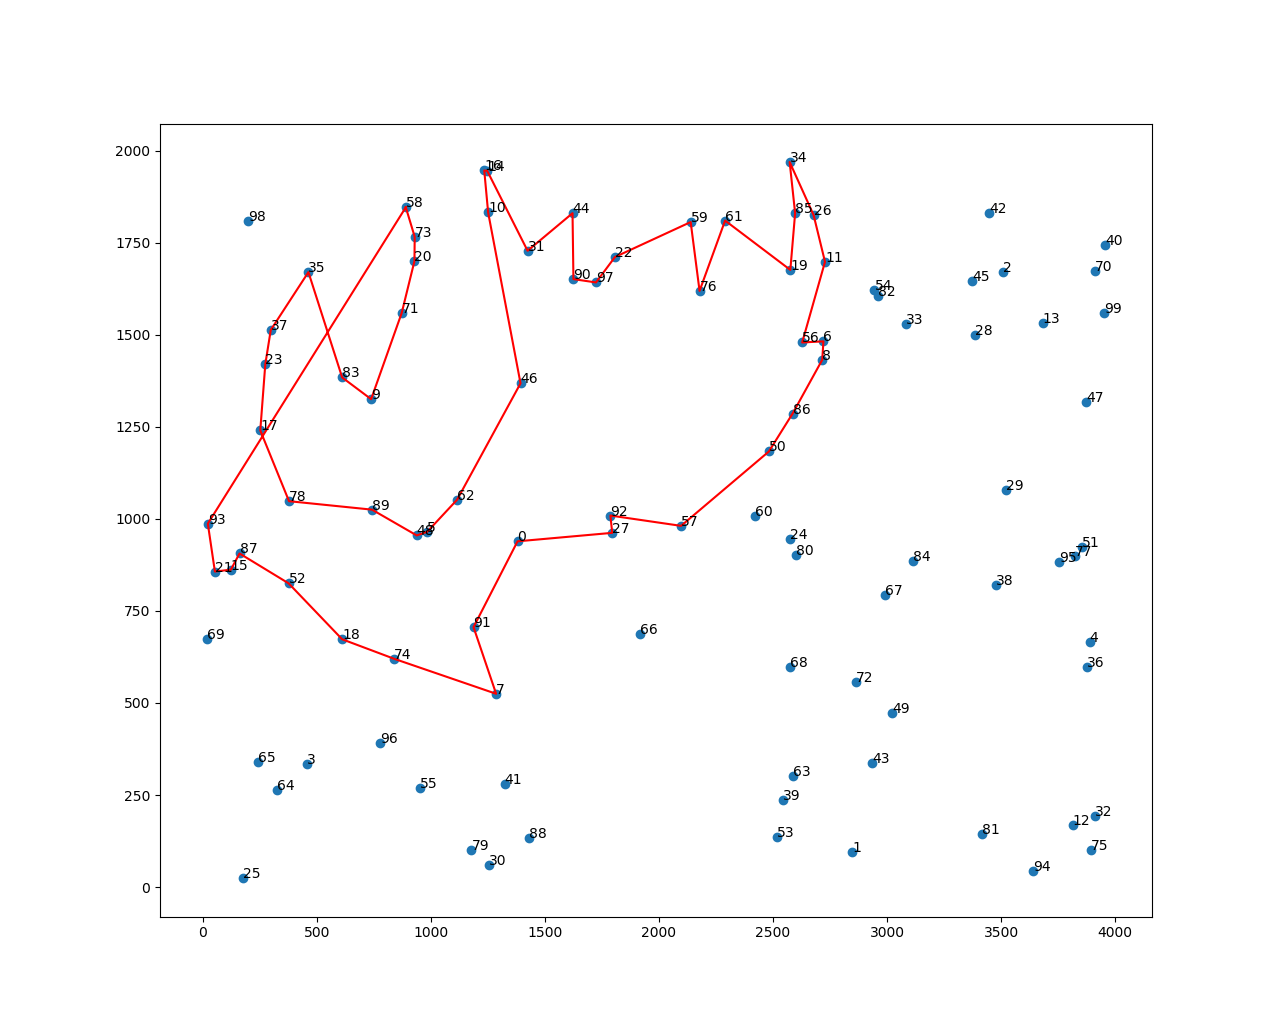
\includegraphics[width=\textwidth]{kroa_greedypng.png}
    \caption{Algorytm zachłanny - KROA100}
  \end{minipage}

  \begin{minipage}[b]{0.8\textwidth}
    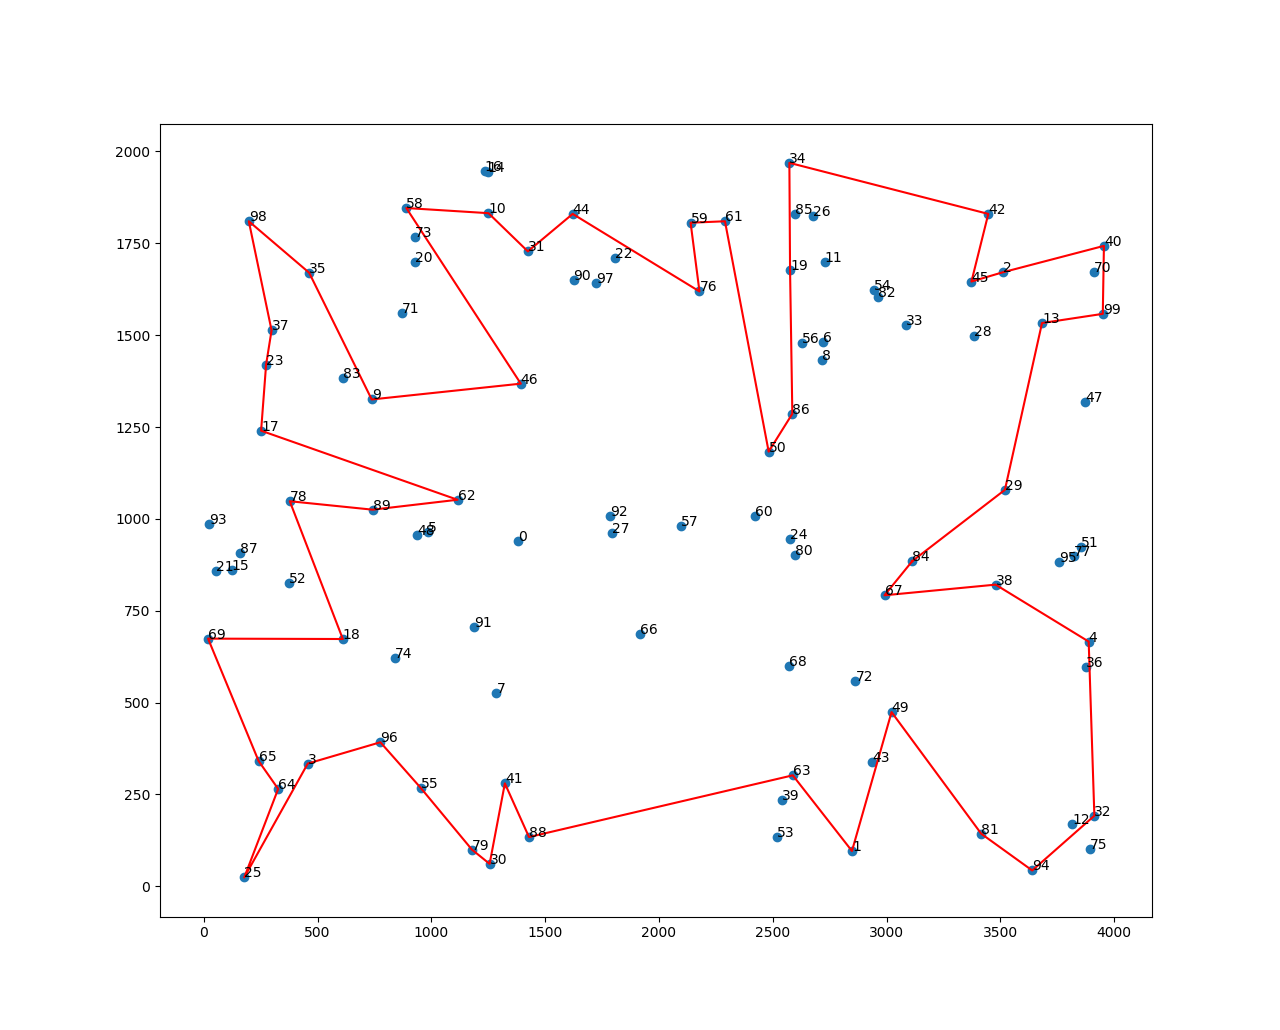
\includegraphics[width=\textwidth]{kroa_min_regret_18679.png}
    \caption{Algorytm z żalem - KROA100}
  \end{minipage}
  
\end{figure}
    
  \begin{figure}[h!]
    \centering
      \begin{minipage}[b]{0.8\textwidth}
        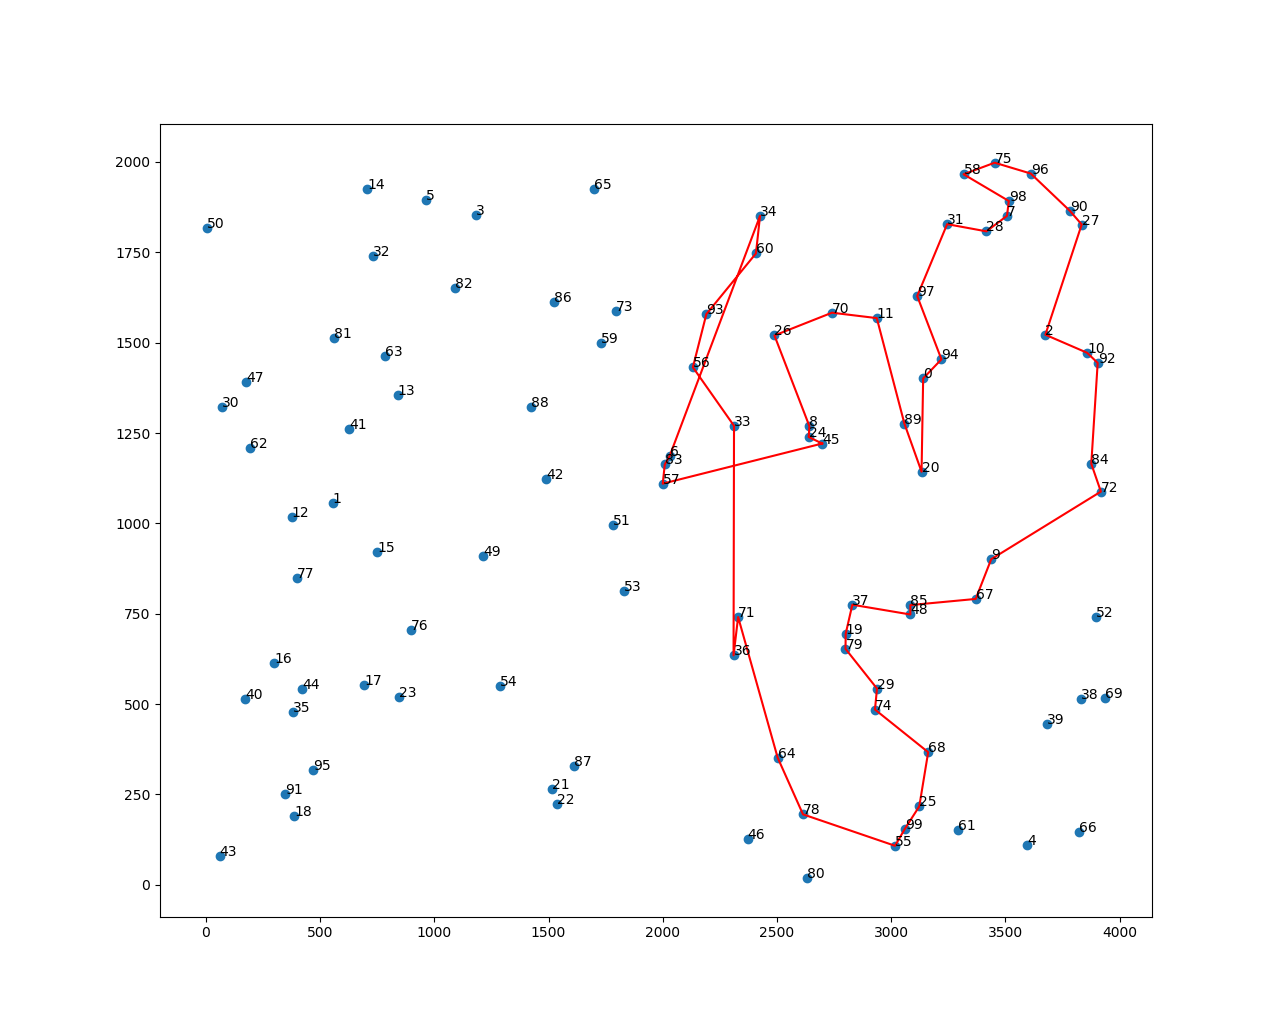
\includegraphics[width=\textwidth]{krob_greedy.png}
        \caption{Algorytm zachłanny - KROB100}
      \end{minipage}
    
      \begin{minipage}[b]{0.8\textwidth}
        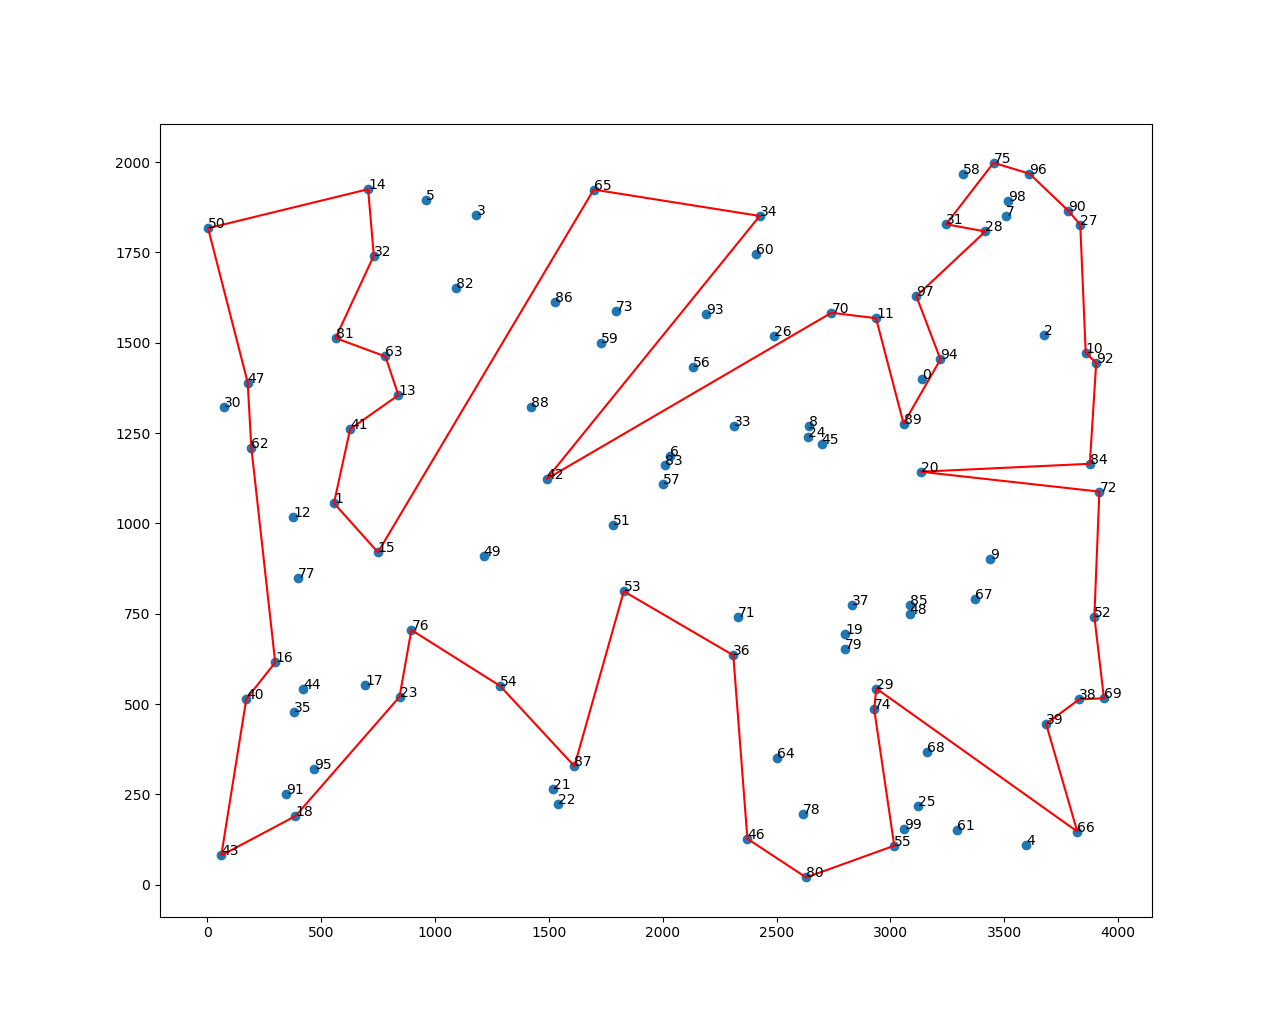
\includegraphics[width=\textwidth]{krob_min_regret_19830.png}
        \caption{Algorytm z żalem - KROB100}
      \end{minipage}  
\end{figure}

\section{Wnioski}

    Wyniki obliczeń jasno wskazują, że algorytm zachłanny radzi sobie znacznie lepiej przy przechodzeniu przez 50\% punktów generując ścieżkę o ok. połowę krótszą. Jednakże kiedy te same algorytmy uruchomi się dla wszystkich punktów, to wyniki są zupełnie inne - algorytm z żalem wyznacza krótsze ścieżki. Dzieje się tak przy uruchamianiu algorytmów dla 90-100\% punktów instancji. Spowodowane jest to tym, że algorytm z żalem wybiera początkowo "gorsze" wierzchołki (z większym żalem, często bardziej oddalone od siebie), co zaczyna przynosić profity dopiero w późniejszym etapie (do którego algorytm nie dochodzi gdyż kończy dodawanie na połowie punktów). Algorytm zachłanny nie ma takiego problemu, jego kontekst "przewidywania" jest węższy, więc przynosi tym lepsze wyniki (w porównaniu do algorytmu z żalem), im mniejsza jest liczba punktów z instancji, którą ma zawierać ścieżka.

\section{Kod programu}

    Repozytorium z kodem algorytmów dostępne jest pod: \url{https://github.com/bbbrtk/aem}


\end{document}
